% Created 2022-09-29 jue 10:43
% Intended LaTeX compiler: pdflatex
\documentclass[11pt]{article}
\usepackage[utf8]{inputenc}
\usepackage[T1]{fontenc}
\usepackage{graphicx}
\usepackage{grffile}
\usepackage{longtable}
\usepackage{wrapfig}
\usepackage{rotating}
\usepackage[normalem]{ulem}
\usepackage{amsmath}
\usepackage{textcomp}
\usepackage{amssymb}
\usepackage{capt-of}
\usepackage{hyperref}
\usepackage[spanish, ]{babel}
\documentclass[12pt]{article}
\renewcommand\familydefault{\sfdefault}
\usepackage[a5paper,left=17mm,right=20mm,top=20mm,bottom=20mm]{geometry}
\usepackage{mdframed}
\BeforeBeginEnvironment{minted}{\begin{mdframed}}
\AfterEndEnvironment{minted}{\end{mdframed}}
\setcounter{secnumdepth}{2}
\author{Luis Eduardo Galindo Amaya}
\date{27-09-2022}
\title{Notas de la Clase}
\hypersetup{
 pdfauthor={Luis Eduardo Galindo Amaya},
 pdftitle={Notas de la Clase},
 pdfkeywords={},
 pdfsubject={},
 pdfcreator={Emacs 26.3 (Org mode 9.1.9)}, 
 pdflang={Sp}}
\begin{document}

\maketitle
\setlength\parindent{0pt}
\tableofcontents
\pagebreak


\section{Trayectoria de datos}
\label{sec:org2aabb80}
Camino de los datos en una máquina von Neumann típica. Los registros almacenan datos temporalmente. Los registros son usados como entradas de la ALU. La ALU genera una operación sobre los registros. El resultado de la operación vuelve a ser almacenado en los registros.

\begin{figure}[htbp]
\centering
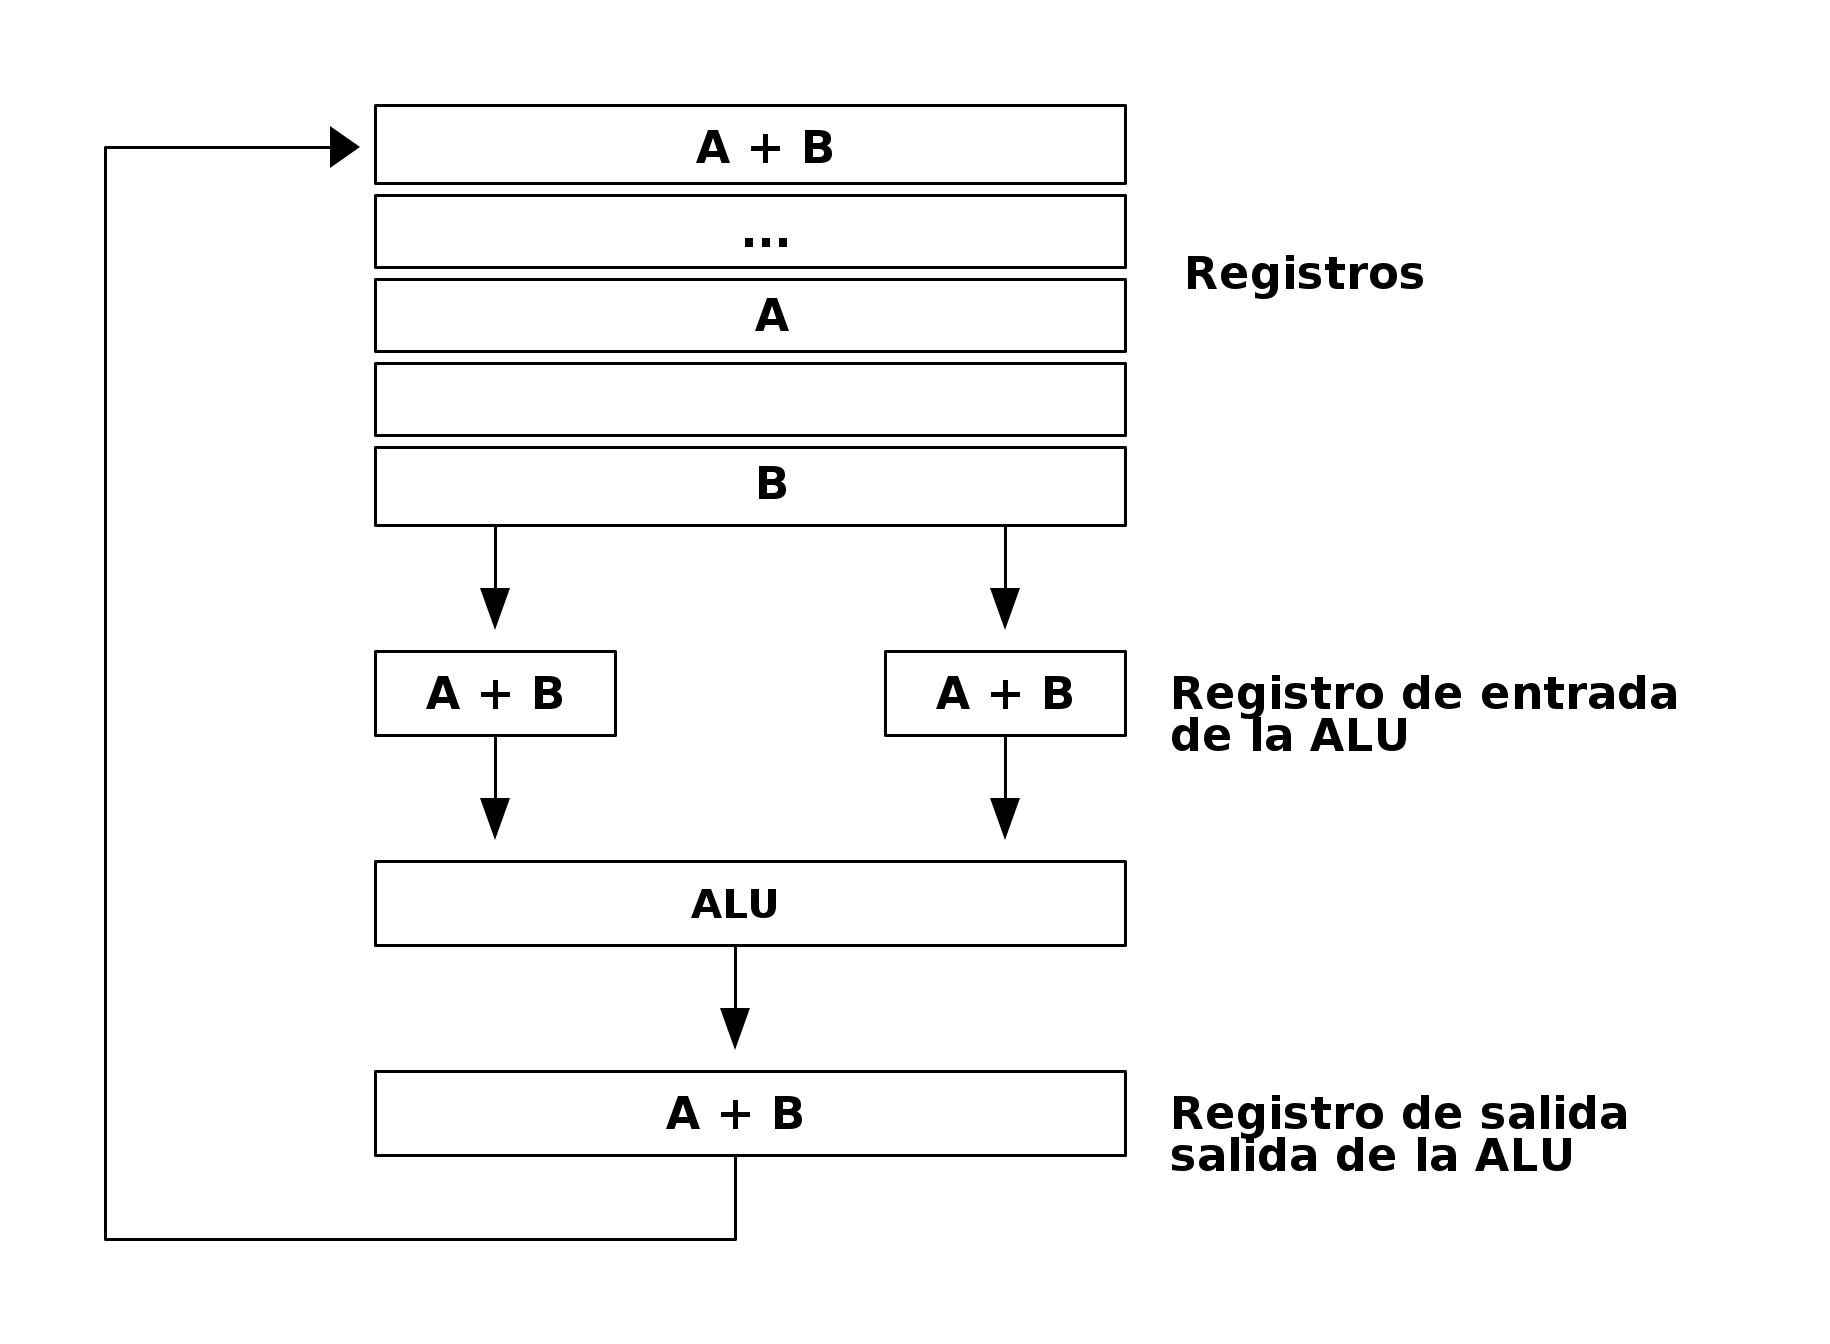
\includegraphics[width=7cm]{./img/trayectoria.png}
\caption{Camino de datos en una arquitectura de Von neuman.}
\end{figure}

\section{Organización de un sistema computarizado}
\label{sec:orgd380676}
\begin{itemize}
\item Las bases que conforman un sistema computarizado son:
\begin{itemize}
\item La Unidad Central de Procesamiento (CPU)
\item La sección de Memoria
\item La sección de Entrada/Salida (E/S)
\end{itemize}

\item Estas tres secciones están interconectadas por tres conjuntos de líneas paralelas llamadas buses o ductos.

\item Estos buses son:
\begin{itemize}
\item Bus de Direcciones
\item Bus de Datos
\item Bus de Control
\end{itemize}
\end{itemize}

\section{Funciones de una computadora}
\label{sec:org8c094fa}
\begin{description}
\item[{Procesamiento de datos}] Los datos pueden adoptar una gran variedad de formas, y el rango de los requisitos de procesado es amplio.

\item[{Almacenamiento de datos}] La computadora tiene que guardar temporalmente al menos aquellos datos con los que está trabajando en un momento dado.

\item[{Transferencia de datos}] El entorno de operación del computador se compone de dispositivos que sirven bien como fuente o bien como destino de datos.

\item[{Control}] Dentro del computador, una unidad de control gestiona los recursos del computador y dirige las prestaciones de sus partes funcionales en respuesta a estas instrucciones.
\end{description}

\section{Diagrama de bloques de una computadora}
\label{sec:orga4ad0e1}
\begin{center}
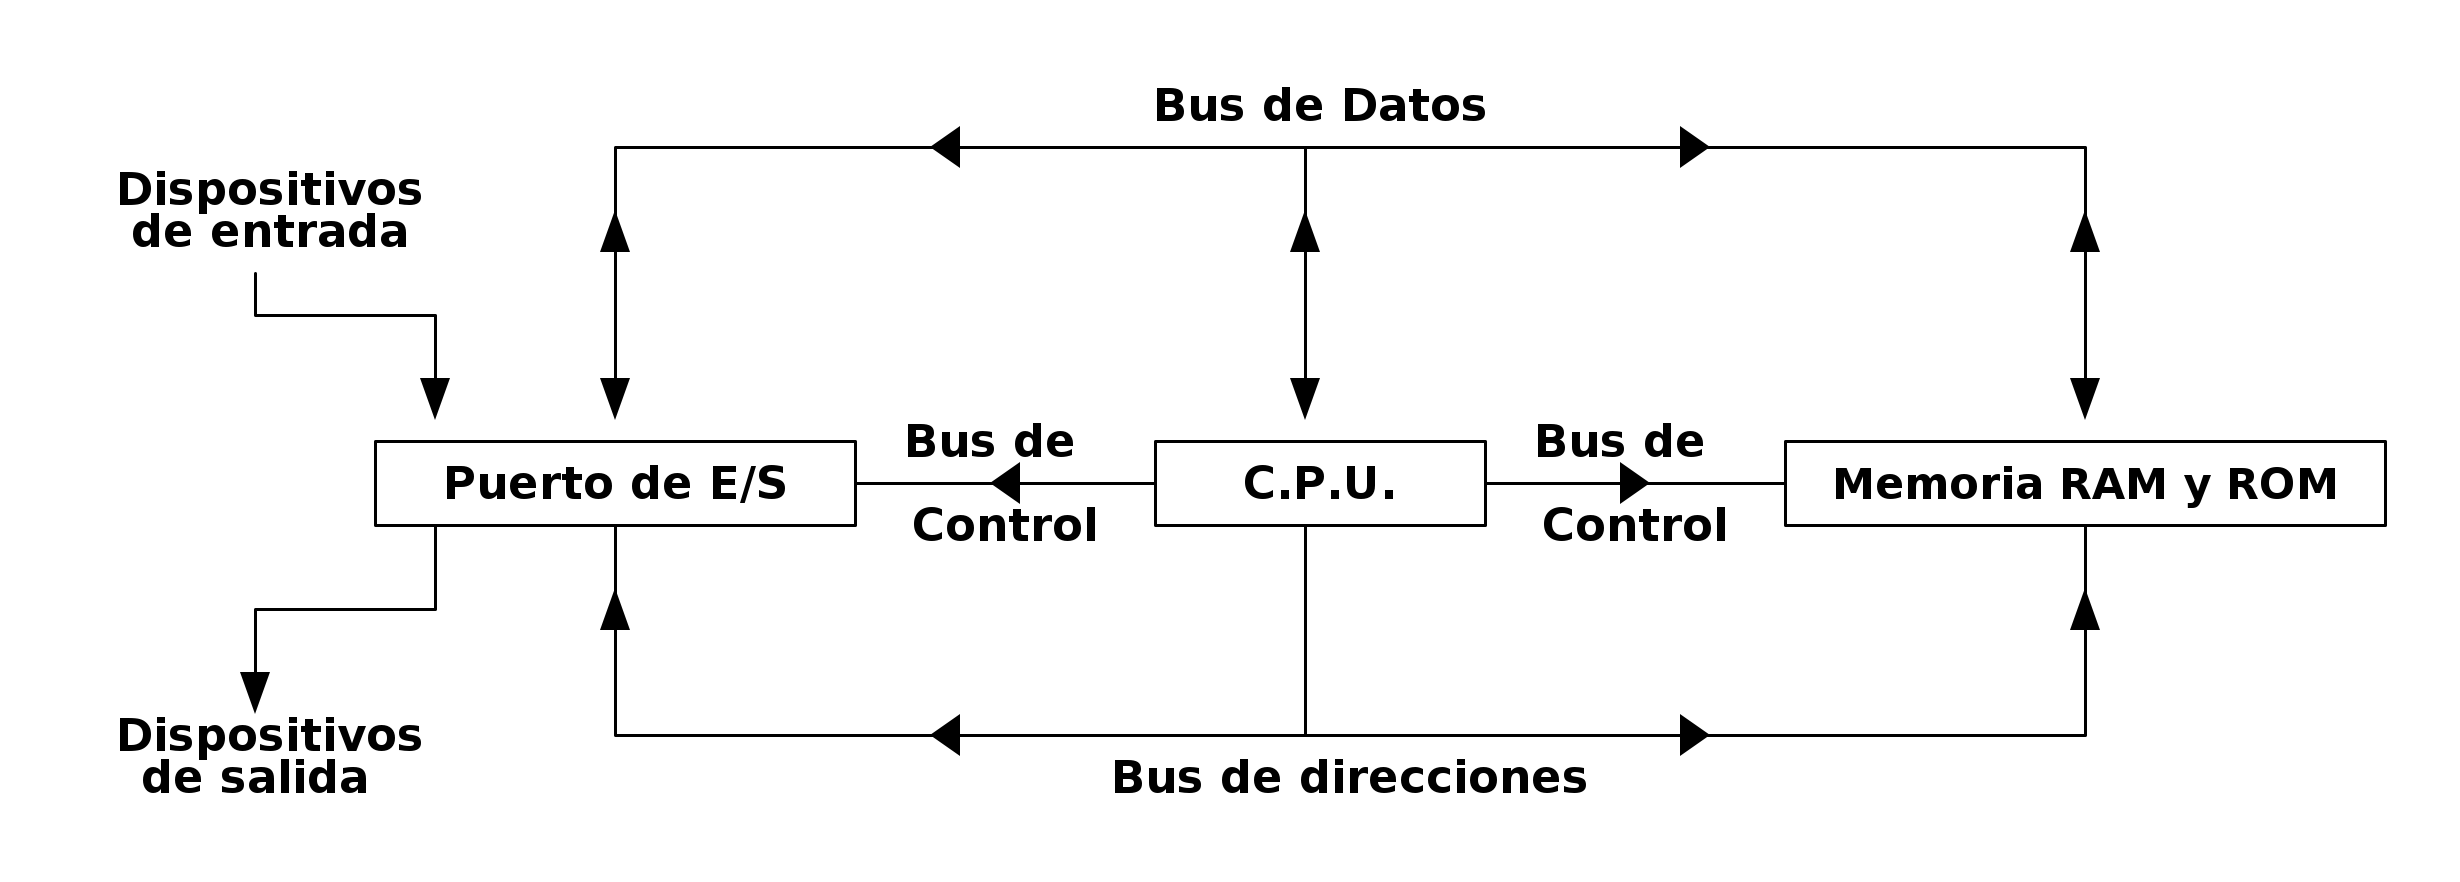
\includegraphics[width=.9\linewidth]{./img/diagramadebloques.png}
\end{center}

\begin{itemize}
\item El CPU \textbf{MANDA} direcciones a través del bus de direcciones a los puertos y a la memoria.

\item El CPU \textbf{MANDA Y RECIBE} datos desde y hacia los puertos y memoria a través del bus de datos.

\item \textbf{MANDA} señales de control a los puertos y memoria, a través del bus de control.
\end{itemize}

\section{Unidad Central de Procesamiento (CPU)}
\label{sec:org2ee81dc}
\subsection{Componentes de CPU}
\label{sec:orgbd129ac}
\begin{itemize}
\item Controla las operaciones del sistema computarizado, \textbf{trae el código binario de las instrucciones} desde la memoria, \textbf{decodifica} las instrucciones a una serie de acciones simples y \textbf{ejecuta} tales acciones.

\item El CPU contiene una \textbf{unidad aritmética y lógica (ALU)}, la cual realiza operaciones como sumar, restar, or, and, xor, invertir etc., sobre palabras binarias, cuando las instrucciones así lo requieran.

\item El CPU también contiene un contador de direcciones o \textbf{Contador de Programa} el cual se utiliza para retener la dirección de la próxima instrucción a ser traída desde la memoria.

\item Además contiene \textbf{registros de propósito general} los cuales se utilizan para almacenar temporalmente datos binarios, y una \textbf{circuitería de control} que genera las señales del bus de control.
\end{itemize}

\subsection{Funciones principales del CPU}
\label{sec:orgbe77135}
\begin{itemize}
\item Seleccionar, decodificar y ejecutar instrucciones de programa en el orden adecuado.

\item Transferir datos hacia y desde la memoria, y hacia y desde las secciones de E/S.

\item Responder a interrupciones externas.

\item Proporcionar las señales de control y de tiempo necesarias para la totalidad del sistema
\end{itemize}

\section{Jerarquía de Memoria}
\label{sec:org3ffa739}
La jerarquía de memoria se emplea para encontrar un balance entre los usos de memorias, para mantener los costos bajos, sin necesidad de sacrificar el rendimiento del sistema.

\begin{center}
\begin{tabular}{|l|l|}
\hline
Inboard memory & Registers\\
 & Cache\\
 & Main memory\\
\hline
Outboard storage & Magnetic disk\\
 & CD-ROM\\
 & CD-RW\\
 & DVD-RW\\
 & DVD-RAM\\
 & Blu-Ray\\
\hline
Off-line storage & Magnetic Tape\\
\hline
\end{tabular}
\end{center}

\section{Paginación de memoria (Probablemente no venga)}
\label{sec:org0286fb4}
\begin{itemize}
\item Los pedazos de un programa, conocidos como páginas, pueden ser asignados a pedazos de memoria conocidos como frames.

\item La memoria principal es dividida en varios pequeños frames de mismo tamaño. Cada proceso es dividido en varias páginas, procesos más pequeños requieren menos páginas, procesos más grandes requieren más páginas.

\item El S.O. mantiene una lista de frames libres.

\item Así se reduce el espacio de memoria desperdiciado.
\end{itemize}

\section{Arquitectura de la computadora}
\label{sec:orge0c0def}
\subsection{Sección de Entrada/Salida}
\label{sec:org03436c2}
Permite a la computadora tomar datos del mundo real o mandar datos al
mundo real. Los periféricos tales como teclados, pantalla e impresoras se
conectan a la sección de E/S.

\subsection{Bus de direcciones}
\label{sec:orga61bff8}
El bus de direcciones son las lineas de cobre dentro del procesador. Dependiendo de la cantidad de lineas que tenga podremos saber el tamaño de las dirección de memoria máxima direccionable.

El bus de direcciones consiste de 16,20,24 o mas líneas de señales en
paralelo. Por estas líneas el CPU envía la localidad de memoria en la
cual va escribir o leer.

El número de localidades que el CPU puede direccionar o acceder se
determina por el número de líneas del bus de direcciones. Si el CPU
tiene N líneas de dirección entonces puede direccionar \(2^N\) localidades.

\begin{figure}[htbp]
\centering
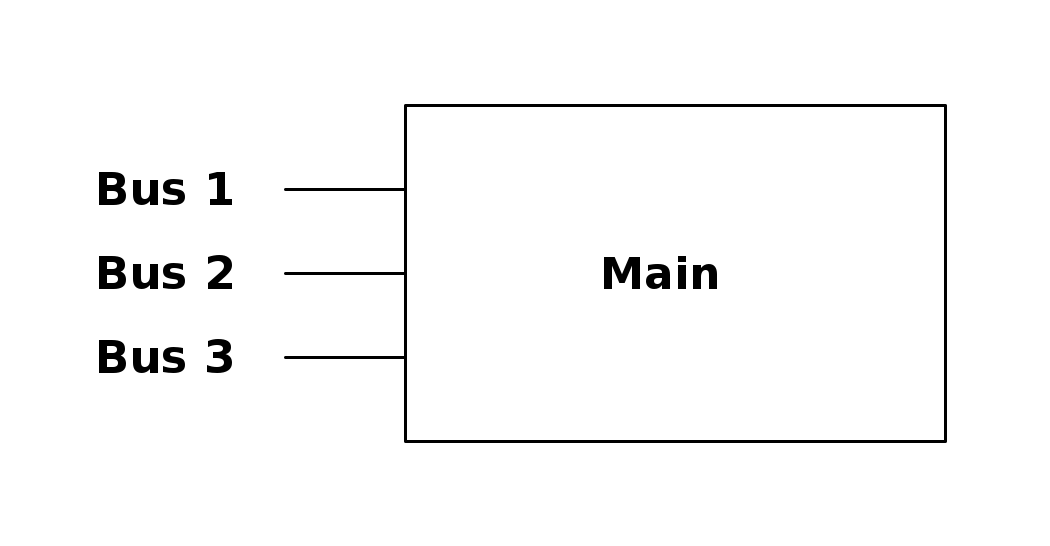
\includegraphics[width=5cm]{./img/busdirecciones.png}
\caption{\(2^3\) direcciones máximas direccionables.}
\end{figure}

\subsection{Bus de datos}
\label{sec:org0d272cd}
El bus de datos consiste de 8,16, 32 o más líneas de señales en paralelo, estas líneas son bidireccionales. Esto significa que el CPU puede leer datos por estas líneas desde la memoria o un puerto así también puede mandar datos a una localidad de memoria o a un puerto. 

Muchos dispositivos en un sistema pueden tener sus salidas conectadas al bus de datos, pero solamente uno puede estar habilitado a la vez. Por lo que cualquier dispositivo conectado al bus de datos debe ser de tres estados de forma que los dispositivos que no estén en uso estén flotados.

\begin{description}
\item[{Resumen}] el bus de datos es bidireccional, puede dar y recibir datos el bus de datos es trifásico\footnote{Que tiene tres estados.} Leyendo, escribiendo y esperando.
\end{description}

\subsection{Bus de Control}
\label{sec:orgc54395b}
\begin{itemize}
\item El bus de control consiste de 4 a 10 líneas de señales en paralelo. El CPU manda señales sobre el bus de control para habilitar las salidas de los dispositivos de memoria o puertos direccionados

\item Generalmente las señales del bus de control son leer memoria, escribir en memoria, leer E/S y escribir E/S.
\end{itemize}

\section{Diferencias de CISC con RISC}
\label{sec:org149842c}
\subsection{CISC}
\label{sec:org117d22b}
\begin{itemize}
\item Una computadora con una gran cantidad de instrucciones se clasifica como una Computadora de Conjunto de Instrucciones Complejo, CISC (Complex Instruction Set Computer).

\item Durante finales de los años 70 se experimentó con instrucciones muy complejas, posibles gracias al intérprete. Los diseñadores intentaron cerrar la "brecha semántica" entre lo que podían hacer las máquinas y lo que requerían los lenguajes de programación de alto nivel.
\end{itemize}

\subsection{RISC}
\label{sec:orgb5f9206}
\begin{itemize}
\item Al principio de los 80, muchos diseñadores de computadoras recomendaron que las maquinas utilizaran menos instrucciones con fórmulas más sencillas que pudieran ejecutarse con mayor rapidez dentro del CPU, sin tener que utilizar la memoria con tanta frecuencia.

\item Este tipo de computadoras se clasifica como Computadoras de Conjunto de Instrucciones Reducido, RISC (Reduced Instructions Set Computers).

\item El concepto de la arquitectura RISC significa un intento para reducir el tiempo de ejecución al simplificar el conjunto de instrucciones de la computadora.
\end{itemize}

\subsection{Tabla de diferencias}
\label{sec:org98ef92f}
\subsubsection*{RISC}
\label{sec:org619e519}
\begin{mdframed}
\begin{itemize}
\item Instrucciones sencillas en un ciclo
\item Cualquier instrucción puede referenciar a memoria
\item Procesamiento serie de varias etapas
\item Instrucciones ejecutadas por hardware
\item Instrucciones de formato fijo
\item Pocas instrucciones y modos
\item La complejidad está en el compilador
\item Varios conjuntos de registros
\end{itemize}
\end{mdframed}

\subsubsection*{CISC}
\label{sec:org814419c}
\begin{mdframed}
\begin{itemize}
\item Instrucciones complejas en varios ciclos
\item Solo LOAD/STORE hacen referencia a memoria
\item Poco procesamiento en serie
\item Instrucciones interpretadas por un microprograma
\item Instrucciones de formato variable
\item Muchas instrucciones y modos
\item La complejidad está en el microprograma
\item Un solo conjunto de registros
\end{itemize}
\end{mdframed}

\section{Arquitectura de Von Neuman}
\label{sec:org9774b8f}
En la arquitectura Von Neumann el programa y los datos están almacenados en la misma memoria.

\begin{center}
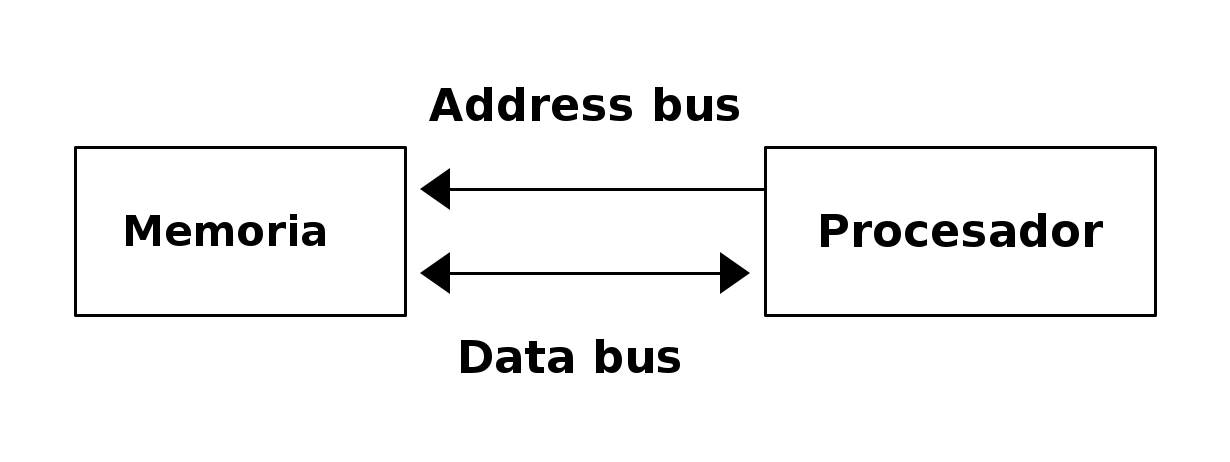
\includegraphics[width=7cm]{./img/vonneuman.png}
\end{center}

\section{Arquitectura de Harvard}
\label{sec:orga9009c4}
En la arquitectura Harvard se manejan espacios de memoria separados para almacenar las instrucciones del programa y los datos, por lo que ambas memorias pueden ser accedidas simultáneamente.

\begin{center}
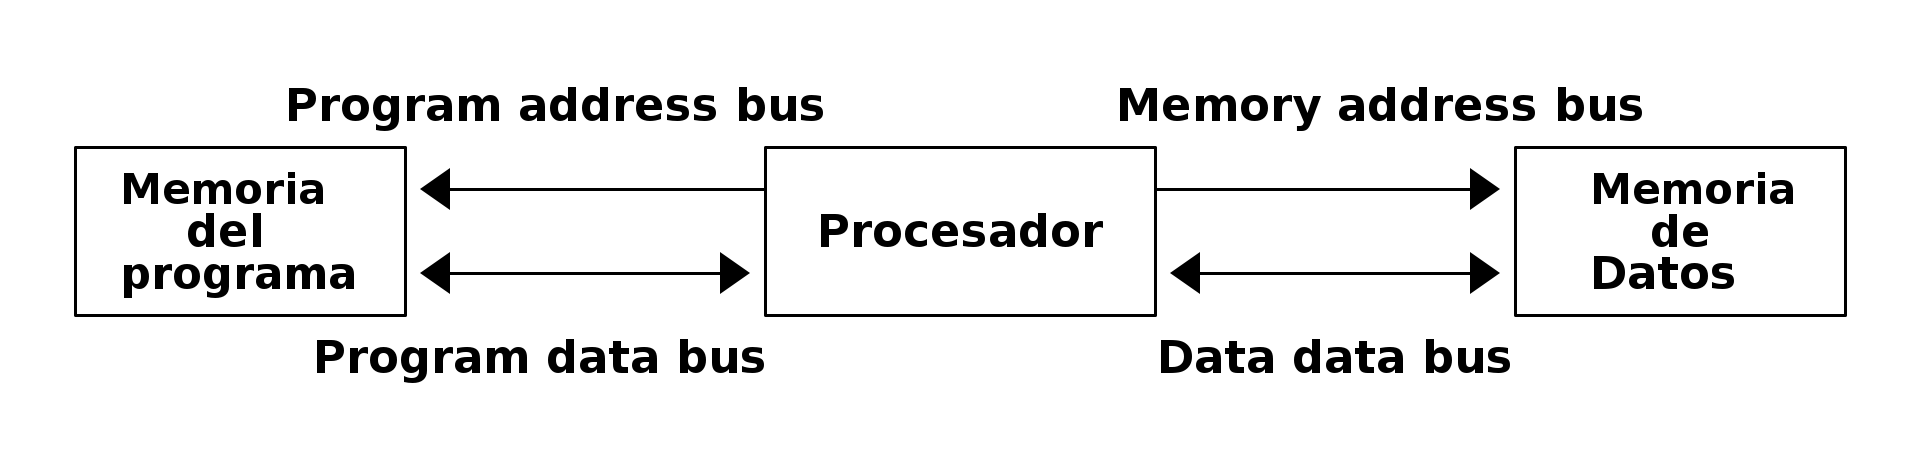
\includegraphics[width=.9\linewidth]{./img/harvard.png}
\end{center}

\section{Taxonomía de Flynn}
\label{sec:org69f832c}
\begin{center}
\begin{tabular}{|l|l|l|}
\hline
 & Single Instruction & Multiple instructions\\
\hline
Single data & SISD & MISD\\
\hline
Multiple data & SIMD & MIMD\\
\hline
\end{tabular}
\end{center}

\section{Sistema de numeración binario}
\label{sec:org73f3917}
\subsection{Conversión de binario a decimal}
\label{sec:org542ac2d}
El sistema de numeración binario solo consiste de dos símbolos 1 y 0, cada posición corresponde a un exponente numero potencia de 2.

\begin{center}
\begin{tabular}{|r|r|r|r|r|l|r|}
\hline
\(2^4=16\) & \(2^3=8\) & \(2^2=4\) & \(2^1=2\) & \(2^0=1\) & \# & DEC\\
\hline
1 & 0 & 1 & 1 & 1 & = & 23\\
\hline
\end{tabular}
\end{center}

\subsection{Conversión decimal a binario}
\label{sec:org86d680b}
Se divide el numero entre 2 y se obtiene su modulo, el resultante del modulo corresponde a cada posición del numero, ejemplo de convertir 200 a binario:

\begin{center}
\begin{tabular}{|l|r|r|r|r|r|r|r|r|}
\hline
n & 200 & 100 & 50 & 25 & 12 & 6 & 3 & 1\\
\hline
n/2 & 100 & 50 & 25 & 12 & 6 & 3 & 1 & 0\\
n\%2 & 0 & 0 & 0 & 1 & 0 & 0 & 1 & 1\\
\hline
\end{tabular}
\end{center}

\[ (200)_{10} = (11001000)_2 \]

\subsection{Suma binaria}
\label{sec:org1ba5de6}
\begin{verbatim}
              1
   35:  0010 0011
+  10:  0000 1010
  ----------------
   45:  0010 1101
\end{verbatim}

\subsection{Multiplicación binaria}
\label{sec:orgbd88272}
\begin{verbatim}
25:      0001 1001   
 3:      0000 0011
         ---------
         0001 1001  <-  se multiplica 1 por 25  
    ...0 0011 001.  <-  otra vez, pero desplazado
    --------------
75:      0100 1011  <- se suman los valores 
\end{verbatim}

\subsection{División entre números binarios}
\label{sec:org2abb805}
\subsubsection*{75/5 = 15}
\label{sec:org997908e}
\begin{verbatim}
         1111                 02           0222
    +------------             1001         1000
101 | 1001011               -  101       -  101  
       101                   ------       ------    
    -------------              100         0011
       1000
        101
    -------------
        0111                  1
         101                  2
    -------------             4
         0101              +  8
          101               ----
    -------------            15 
          000
\end{verbatim}

\subsection{Números negativos en binario}
\label{sec:org7e1e410}
\subsubsection*{Representación en signo-magnitud}
\label{sec:org05fd12e}
El bit mas significativo representa el tipo de números, 1 es negativo y 0 es positivo.

\subsubsection*{Complemento a 1}
\label{sec:org8d92fac}
Niega los valores de los bits, entonces los '0' se vuelven '1' y los '1' se vuelven '0':

\begin{verbatim}
BIN: 1000101010111  ->  CMP1: 0111010101000
\end{verbatim}

\subsubsection*{Complemento a 2}
\label{sec:org1d13dc8}
Es una manera de representar los valores negativos esta representación resuelve el problema del doble cero, pero ahora sus rangos no son iguales en ambas direcciones\footnote{También utiliza el bit más significativo como bit de signo.}:

\begin{mdframed}
El rango de números representables en el sistema de complemento a 2 va desde \(-(2^{n-1})\) hasta \(+(2^{n-1} - 1)\), donde 'n' es el numero de bits.
\end{mdframed}

para convertir un numero binario a su complemento a 2, solamente calculamos su complemento a 1 y le sumamos 1:

\begin{verbatim}
Convertir 5 a CMP2         Convertir -5 a BIN

    5: 0000 0101              -5: 1111 1011 - 1
 CMP1: 1111 1010 + 1        CMP1: 1111 1010
 CMP2: 1111 1011             BIN: 0000 0101 = 5
\end{verbatim}

\subsubsection*{Suma de complemento 2}
\label{sec:org9548b8c}
Si sumamos un numero positivo a un complemento a 2 el equivalente a hacer la resta de los números.

\begin{verbatim}
         1111 111 
 5: .... 0000 0101     Como nuestra operación esta
-5: .... 1111 1011     fija a 8 bits, el resultado 
    --------------     es correcto, a pesar de que 
    ...1 0000 0000     tiene desbordameniento
\end{verbatim}

\subsubsection*{Errores de sobreflujo}
\label{sec:org489b142}
\begin{mdframed}
El sobreflujo solo sucede cuando al sumar dos números con el mismo signo, el resultado nos resulta con signo contrario.
\end{mdframed}

\begin{verbatim}
     No overflow               Overflow

          11   111                1       
   -75:   1011'0101        -92:   1010'0100
+  -25:   1110'0111     +  -40:   1101'1000 
  ------------------      ------------------      
  -100: 1'1001'1100       -132: 1'0111'1100
\end{verbatim}

\begin{description}
\item[{No overflow}] A pesar de que el valor abarca in bit extra para la operacion el signo coincide con los valores de la suma, por lo que no hay overflow.

\item[{Overflow}] Por otra parte para solucionar este caso es necesario un bit extra para representalo y el bit de signo es diferente a los operadores, por lo tanto ha y sobreflujo.
\end{description}

\subsection{Representación decimal a binario}
\label{sec:org42033a1}
76.875 ,Para la parte entera de la división hacemos la división como normalmente la hacemos, dividiendo entre 2 y obteniendo el modulo\footnote{En clase no vimos ningún caso con decimal periódico, pero en caso de venir el resultado esta limitado por la cantidad de bits disponible.}.

\begin{center}
\begin{tabular}{|l|r|r|r|r|r|r|r|}
\hline
n & 76 & 38 & 19 & 9 & 4 & 2 & 1\\
\hline
n/2 & 38 & 19 & 9 & 4 & 2 & 1 & 0\\
n\%2 & 0 & 0 & 1 & 1 & 0 & 0 & 1\\
\hline
\end{tabular}
\end{center}

Ahora para obtener la parte decimal es necesario que multipliquemos por 2, si el resultado tiene un entero lo eliminamos y lo usamos como el valor binario

\begin{center}
\begin{tabular}{|l|r|r|r|}
\hline
n & .375 & .75 & .50\\
\hline
n*2 & 0.75 & 1.5 & 1\\
int & 0 & 1 & 1\\
\hline
\end{tabular}
\end{center}

\[76.375_{10} = 1001100.011_2\]

\subsection{Binario con punto decimal a flotante}
\label{sec:orge3d9823}
1001100.011, Simplemente extendemos nuestra tabla de exponentes con los números negativos\footnote{\(x^{-n} = \frac{1}{x^n}\)}

\begin{center}
\begin{tabular}{|l|r|r|r|r|r|r|r|l|r|r|r|}
\hline
exp & 6 & 5 & 4 & 3 & 2 & 1 & 0 &  & -1 & -2 & -3\\
\hline
 & 1 & 0 & 0 & 1 & 1 & 0 & 0 & . & 0 & 1 & 1\\
\hline
\end{tabular}
\end{center}

\[
2^{6} + 2^{3} + 2^{2} + 2^{-1} + 2^{-2} + 2^{-3}
\]

\[
64 + 8 + 4 + 0.5 + 0.25 + 0.125 = \boxed{76.875}
\]

\subsection{BCD (Binary Coded Decimal)}
\label{sec:org7e12fca}
El BCD sirve para representar los números decimales de manera sencilla en código binario, cada sección del código corresponde a un dígito de nuestro numero:

\begin{verbatim}
 19 -> 1: 0001 9: 1001
130 -> 1: 0001 3: 0011 0: 0000
\end{verbatim}

\section{Sistema Hexadecimal}
\label{sec:orgda8f093}
\subsection{Ventajas}
\label{sec:org2f05cc3}
Este sistema es base 16 por lo que usamos letras para representar los números:

\begin{center}
\begin{tabular}{|r|r|r|r|r|r|r|r|r|r|r|r|r|r|r|r|}
\hline
0 & 1 & 2 & 3 & 4 & 5 & 6 & 7 & 8 & 9 & 10 & 11 & 12 & 13 & 14 & 15\\
\hline
0 & 1 & 2 & 3 & 4 & 5 & 6 & 7 & 8 & 9 & A & B & C & D & E & F\\
\hline
\end{tabular}
\end{center}

\subsubsection*{Las principales ventajas de este sistema son:}
\label{sec:orgd2634ce}
\begin{itemize}
\item Puede representar números muy grandes en menos espacio.
\item Un nibble (4 bits) se pueden representar con un solo valor.
\end{itemize}

\begin{center}
\begin{tabular}{|r|l|l|}
\hline
Decimal & Binario & Hexadecimal\\
217 & 1101 1001 & D9\\
\hline
\end{tabular}
\end{center}

\subsection{Conversión decimal a hexadecimal}
\label{sec:org8d12ec8}
Dividimos entre 16 y obtenemos el modulo, el modulo es el valor que corresponde al numero hexadecimal

\begin{center}
\begin{tabular}{|l|r|r|r|r|}
\hline
n & 5000 & 312 & 19 & 1\\
\hline
n/16 & 312 & 19 & 1 & 0\\
n\%16 & 8 & 8 & 3 & 1\\
hex(n\%16) & 8 & 8 & 3 & 1\\
\hline
\end{tabular}
\end{center}

\[ 5000_{10} = 1388_{16} \]

\subsection{Conversión hexadecimal a decimal}
\label{sec:orgfb88632}
Reemplazamos el valor hexadecimal con su valor decimal, lo multiplicamos por \(16^n\) donde 'n' es la posición:

\[ A5A5_{16} = 10*16^3 + 5*16^2 + 10*16 + 5 = 42405_{10} \]

\subsection{Conversión binario a hexadecimal}
\label{sec:org6d7bb68}
\begin{verse}
Un nibble (4 bits) se pueden representar con un solo valor hexadecimal.\\
\end{verse}

Por lo tanto solo tenemos que separar el numero en secciones de 4 bits y sustituir el valor por su correspondiente valor hexadecimal:

\begin{verbatim}
BIN: 1001 1101 1111 0000 
DEC:    9   14   15    0
HEX:    9    E    F    0 -> 0x9EF0
\end{verbatim}

Para convertir el binario a hexadecimal basta con hacer el mismo proceso pero a la inversa, convertimos cada dígito en su correspondiente valor binario y lo concatenamos 

\begin{verbatim}
HEX:    9    E    F    0 
BIN: 1001 1101 1111 0000 -> 1001110111110000
\end{verbatim}

\section{Números flotantes}
\label{sec:org66c89ea}
\subsection{Distribución de bits de un numero flotante}
\label{sec:org2729c53}
\subsubsection*{Precisión simple}
\label{sec:org3782412}
\begin{center}
\begin{tabular}{|l|r|r|r|}
\hline
 & Signo & Exponente & Matiza\\
\hline
Bits & 1 & 8 & 23\\
\hline
\end{tabular}
\end{center}

\subsubsection*{Doble Precisión}
\label{sec:orgd6789be}
\begin{center}
\begin{tabular}{|l|r|r|r|}
\hline
 & Signo & Exponente & Matiza\\
\hline
Bits & 1 & 11 & 52\\
\hline
\end{tabular}
\end{center}

\subsection{Convertir decimal a binario}
\label{sec:org9c0edf1}
\subsubsection*{Convertir flotante a decimal}
\label{sec:orgff3c4e2}
\[200.09375\]

\begin{center}
\begin{tabular}{|l|r|r|r|r|r|r|r|r|}
\hline
n & 200 & 100 & 50 & 25 & 12 & 6 & 3 & 1\\
\hline
n/2 & 100 & 50 & 25 & 12 & 6 & 3 & 1 & 0\\
n\%2 & 0 & 0 & 0 & 1 & 0 & 0 & 1 & 1\\
\hline
\end{tabular}
\end{center}

\begin{center}
\begin{tabular}{|l|r|r|r|r|}
\hline
n & 0.09375 & 0.1875 & 0.75 & 0.5\\
\hline
n*2 & 0.1875 & 0.75 & 1.5 & 1\\
int & 0 & 0 & 1 & 1\\
\hline
\end{tabular}
\end{center}

\[11001000.0011_2\]

\subsubsection*{Desplazamientos}
\label{sec:org707e1ea}
tenemos que recorrer el punto hasta que solo quede un numero al inicio, en nuestro caso el numero de desplazamientos es 7, por lo tanto nuestro exponente es 7.

\begin{center}
\begin{tabular}{|r|r|}
\hline
N. Desp. & Numero\\
\hline
0 & 11001000.0011\\
1 & 1100100.00011\\
2 & 110010.000011\\
3 & 11001.0000011\\
4 & 1100.10000011\\
5 & 110.010000011\\
6 & 11.0010000011\\
7 & 1.10010000011\\
\hline
\end{tabular}
\end{center}

\subsubsection*{Calculando el Bias}
\label{sec:orga1d52c9}
El exponente esta representado con números negados por lo que tenemos que hacer el ajuste\footnote{\(2^{n-1} - 1\), donde 'n' es el numero de bits en el exponente.}, en nuestro caso estamos usando precisión simple por lo que se usan 8 bits:

\begin{verbatim}
n (n. de bits) = 8
          bias = 2^(8-1) - 1
          bias = 127
\end{verbatim}

calculamos el valor inverso de nuestro exponente:

\[ N. Desplazamientos + bias = exponente \]

\[ 7 + 127 = 134_{10} \rightarrow \boxed{10000110_2} \]

\subsubsection*{Matiza}
\label{sec:org92e478d}
la matiza es la parte antes del primer uno en nuestra división

\[
1.\underbrace{10010000011}_{\text{Matiza}}
\]

\subsubsection*{Representación binaria}
\label{sec:orge56c2e1}
\begin{center}
\begin{tabular}{|r|l|l|}
\hline
signo & Exponente & Matiza\\
\hline
0 & 1000 0110 & 1001 0000 0011 0000 0000 000\\
\hline
\end{tabular}
\end{center}

\subsection{Convertir representación binario a decimal}
\label{sec:org2ab60e6}

\begin{center}
\begin{tabular}{|r|r|r|}
\hline
signo & Exponente & Matiza\\
\hline
1 & 01111000 & 10001110001110000000000\\
\hline
\end{tabular}
\end{center}

El primer bit indica el signo del numero, en este caso como el numero es '1' valor es negativo.

\subsubsection*{Obtener el exponente}
\label{sec:org09e8b55}
\begin{verbatim}
01111000 = 120

 x + 127 = 120 
       x = 120 - 127
       x = -7
\end{verbatim}

\subsubsection*{Convertir la matiza en decimal}
\label{sec:org55854c8}
Los exponentes son -1, -2, -3\ldots{} hasta llegar al final:

\begin{verbatim}
# solucion en python
matiza = "10001110001110000000000"
a = [ 2**(-(i+1)) for i,v in enumerate(matiza) if v=='1' ]
return sum(a)
\end{verbatim}

\begin{verbatim}
0.5555419921875
\end{verbatim}

\subsubsection*{Flotante final}
\label{sec:org7af99b8}
\(-1 \times 2^{-7} \times (1+0.5555419921875) = -0.01215267181\)

\section{¿Que es un traductor?}
\label{sec:orga802d67}
\begin{itemize}
\item Un traductor es un programa que convierte un programa escrito en un lenguaje a otro lenguaje distinto.

\item Al lenguaje en que esta escrito el programa original se le denomina lenguaje fuente, y al lenguaje al que se traduce se le conoce como lenguaje objeto.

\item Si se contara con un procesador que ejecutara directamente los programas escritos en lenguaje fuente, no sería necesaria la traducción.

\item Los programas tanto el fuente como el objetos son equivalentes desde el punto de vista funcional, es decir, producen los mismos resultados.
\end{itemize}

\section{Traducción vs Interpretación}
\label{sec:org5f3bc04}
\begin{itemize}
\item En la traducción, el programa original en código fuente no es ejecutado directamente. En su lugar, es convertido a un programa equivalente conocido como programa objeto o programa binario ejecutable cuya ejecución comienza solo hasta que la traducción es completada.

\item En la interpretación, solo existe un paso: la ejecución del programa fuente original.
\end{itemize}

\section{Lenguajes de alto y bajo nivel}
\label{sec:orgaf7fd2d}
El termino alto nivel significa que están orientados hacia la gente, en contraste con el lenguaje ensamblador de bajo nivel el cual esta orientado hacia la máquina.

\section{Estructura de una instruccion de ensamblador}
\label{sec:org04322f6}
\begin{description}
\item[{Etiqueta}] El ensamblador define la etiqueta como equivalente a la dirección en el que se cargará el primer byte del código objeto generado para esa instrucción.

\item[{Mnemónico}] Es el nombre de la operación o función del enunciado.

\item[{Operandos}] Una instrucción en lenguaje ensamblador incluye cero o más operandos. Cada operando identifica un valor inmediato, un valor de registro o una ubicación de memoria.

\item[{Comentarios}] Igual que en otros lenguajes.
\end{description}

\subsection{Estructura}
\label{sec:org9a0c1dd}
\begin{verbatim}
ETIQUETA:
  MNEMONICO OPERANDO(S) ;COMENTARIO
\end{verbatim}

\section{Tipos de ensambladores}
\label{sec:org06a955d}
\subsection{de dos pasos}
\label{sec:org65b552b}
\subsubsection*{Primera pasada}
\label{sec:orga4384f9}
\begin{itemize}
\item El ensamblador solo se ocupa de las definiciones de etiquetas.

\item El primer paso se usa para construir una tabla de símbolos que contiene una lista de todas las etiquetas y sus valores de contador de ubicación (LC) asociados.

\item El ensamblador debe analizar cada instrucción lo suficiente como para determinar la longitud de la instrucción de máquina correspondiente y, por lo tanto, cuánto incrementar el LC.
\end{itemize}

\subsubsection*{Segunda pasada}
\label{sec:org927358b}
\begin{itemize}
\item Cada instrucción se traduce al código de máquina binario apropiado. La traducción incluye las siguientes operaciones:
\end{itemize}


\subsection{de un paso}
\label{sec:org017a1ea}
\textbf{Dificultad}: Los operandos de instrucción pueden ser símbolos que aún no se han definido en el programa fuente.

Cuando el ensamblador encuentra un operando de instrucción que es un símbolo que aún no está definido, el ensamblador hace lo siguiente:

\begin{itemize}
\item 1. Deja el campo del operando de la instrucción vacío (todo ceros) en la instrucción binaria ensamblada.

\item 2. El símbolo utilizado como operando se introduce en la tabla de símbolos. La entrada de la tabla está marcada para indicar que el símbolo no está definido.

\item 3. La dirección del campo de operando en la instrucción que hace referencia al símbolo indefinido se agrega a una lista de referencias directas asociadas con la entrada de la tabla de símbolos.
\end{itemize}

\section{Linking (Enlazamiento)}
\label{sec:orgb2fef1b}
\subsection{¿Que es?}
\label{sec:org44ceff5}
El enlazador es un programa que fusiona los espacios de direcciones separados de los módulos de objetos en un único espacio de direcciones.

\subsection{¿Como lo hace?}
\label{sec:orgc938541}
\begin{itemize}
\item 1. Construye una tabla de todos los módulos de objetos y sus longitudes.

\item 2. Con base en esta tabla, asigna una dirección de inicio a cada módulo de objeto.

\item 3. Encuentra todas las instrucciones que hacen referencia a la memoria y agrega a cada una, una constante de reubicación igual a la dirección inicial de su módulo.

\item 4. Encuentra todas las instrucciones que hacen referencia a otros procedimientos e inserta la dirección de estos procedimientos en el lugar
\end{itemize}

\subsection{¿para que lo hace?}
\label{sec:org38d449f}
\begin{mdframed}
Como en ensamblador las etiquetas de salto son posisciones de memoria es necesario ajustarlas par que los metodos en el programa tengan sentido.
\end{mdframed}

En cada módulo de objeto, puede haber referencias de direcciones a ubicaciones en otros módulos. Cada una de estas referencias solo puede expresarse simbólicamente en un módulo de objeto no vinculado. El enlazador crea un único módulo de carga que es la unión contigua de todos los módulos de objetos.
\end{document}
